% explain goal
% explain data set
% show problems data set


\slide{Image Segmentation}
{
% We want to introduce the problem:
%	- Tell about image segmentation
%		Segment image into several classes..?
%	What do we want to tell about image segmentation?
	\begin{columns}
		\begin{column}{.5\textwidth}
			\begin{itemize}
				\item Old books, from 16th and 17th century (Dutch golden age)  are
			scanned and digitally available
				\item For some, the text is available seperately
				\item Goal: extract images to show those seperately as well
			\end{itemize}
		\end{column}
		\begin{column}{.5\textwidth}
			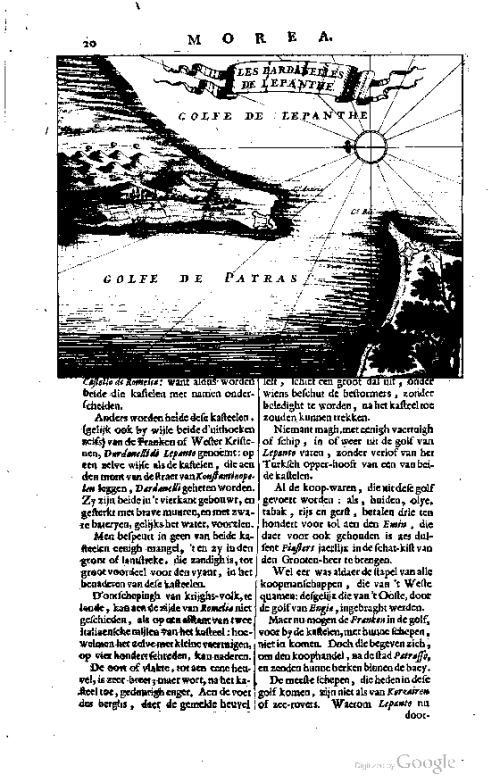
\includegraphics[width=.9\columnwidth]{resources/bookExample}
		\end{column}
	\end{columns}
}

\subsection{Dataset}
\slide{Dataset - Overview 1}
{
	Text pages:
	\begin{columns}
		\begin{column}{.5\textwidth}
			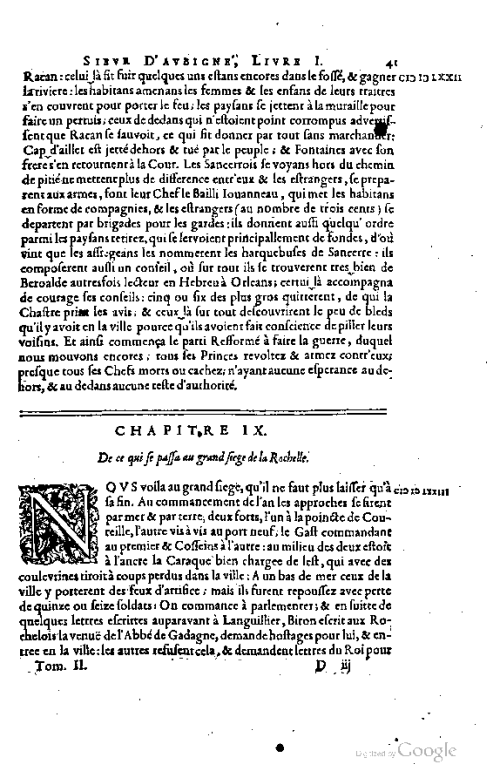
\includegraphics[width=.9\columnwidth]{../data/lhistoireUniverselleDuSieurDavign/raw/500_0043}
		\end{column}
		\begin{column}{.5\textwidth}
			
\includegraphics[width=.9\columnwidth]{../data/lesSixVoyagesDeJeanBaptisteTaverni/raw/500_0010}
		\end{column}
	\end{columns}
}
\slide{Dataset - Overview 2}
{
	Image pages:
	\begin{columns}
		\begin{column}{.5\textwidth}
			
\includegraphics[width=.9\columnwidth]{../data/naukeurigeBeschryvingVanMoreaEertijt/raw/500_0008}
		\end{column}
		\begin{column}{.5\textwidth}
			
\includegraphics[width=.9\columnwidth]{../data/lesSixVoyagesDeJeanBaptisteTaverni/raw/500_0077}
		\end{column}
	\end{columns}
}
\slide{Dataset - Challenge 1}
{
	Difference in quality:
	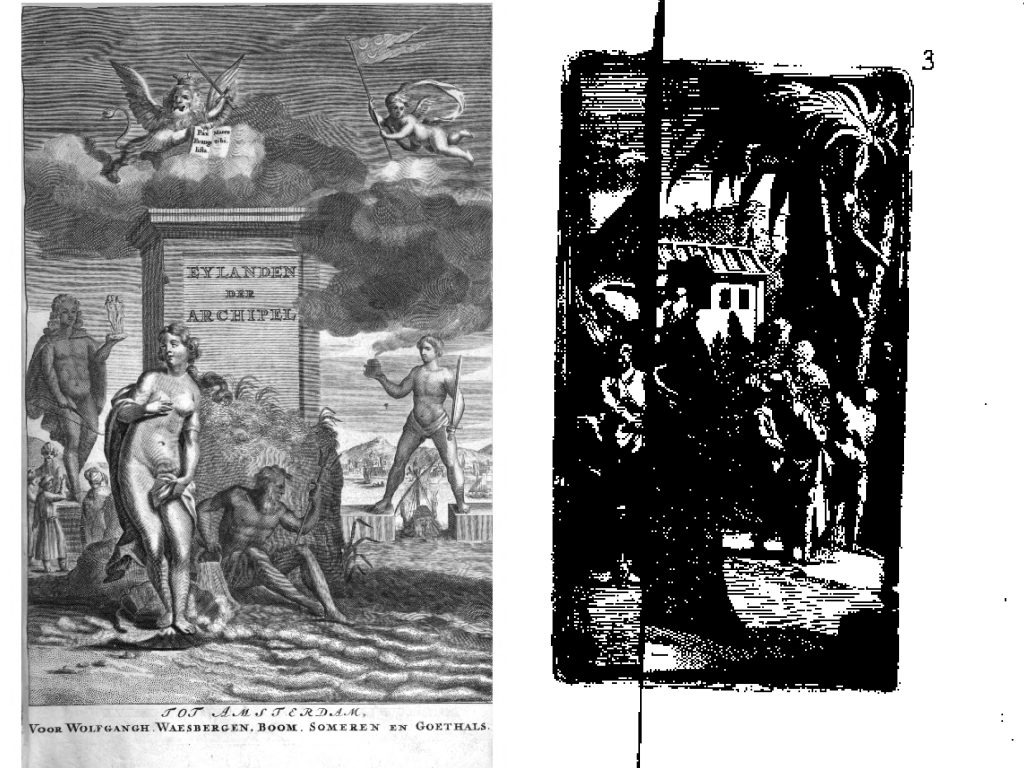
\includegraphics[width=.8\paperwidth]{resources/example2}
}
\slide{Dataset - Challenge 2}
{
	Pages with useless data:
	\begin{columns}
		\begin{column}{.5\textwidth}
			
\includegraphics[width=.9\columnwidth]{../data/staatZugtigeScheepsTogtenEnKrygsBe/raw/500_0002}
		\end{column}
		\begin{column}{.5\textwidth}
			
\includegraphics[width=.9\columnwidth]{../data/atlas/raw/500_0004}
		\end{column}
	\end{columns}
}
\slide{Dataset - Challenge 3}
{
	Text and image on the same page
	\begin{columns}
		\begin{column}{.5\textwidth}
			
\includegraphics[width=.9\columnwidth]{../data/tweeOngelukkigeScheepsTogtenNaOost/raw/500_0003.png}
		\end{column}
		\begin{column}{.5\textwidth}
			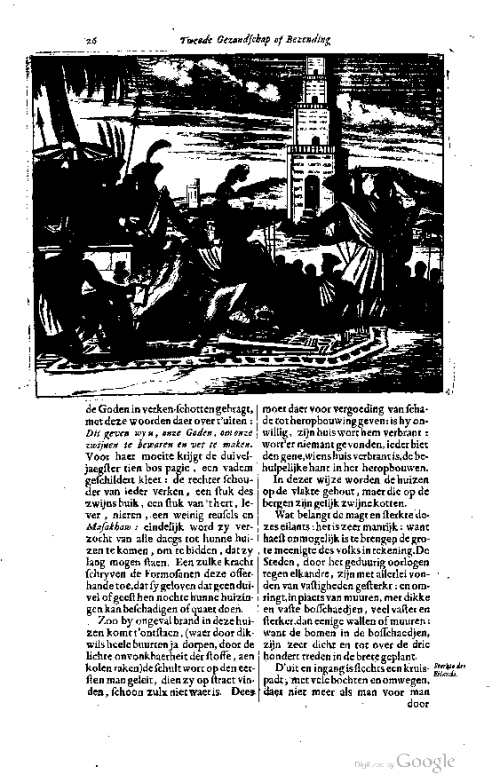
\includegraphics[width=.9\columnwidth]{resources/text_and_image_example}
		\end{column}
	\end{columns}
}

\begin{frame}
\frametitle{Train Set Statistics}

Also a lot of difference in pages and images per book:

\begin{center}
\begin{tabular}{l l}
Total amount of pages: & 5960 \\
Mean pages per book: & 236 \\
Standard deviation: & 223 \\
Total amount of images: & 525 \\
Mean images per book: & 22.8 \\
Standard deviation: & 49.8
\end{tabular}
\end{center}

So we will have to deal with this unfair distribution!

\end{frame}

\subsection{Overview}
\slide{Project Overview - Step 1}
{
	\begin{columns}
		\begin{column}{.4\textwidth}
			Step one: annotate
			\begin{enumerate}
				\item Create annotation tool
				\item Classify page as either `text', `useless' or `containing an image'
				\item Annotate bounding boxes of images
			\end{enumerate}
		\end{column}
		\begin{column}{.6\textwidth}
			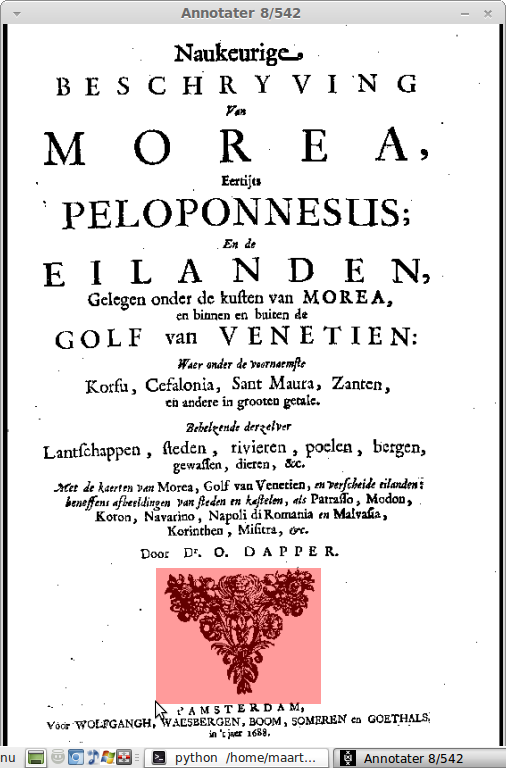
\includegraphics[width=.8\columnwidth]{resources/screenshot_annotator}
		\end{column}
	\end{columns}
}
\slide{Project Overview - Step 2-3}
{
	Step two: classify pages
	\begin{enumerate}
		\item Calculate 5x5 HOG features per page
		\item Train a Support Vector Machine (SVM) on these feature vectors and
		labels
		\item Predict whether a page contains an image based on this SVM
	\end{enumerate}
	Step three: localize images on pages
	\begin{enumerate}
		\item Calculate 10x20 HOGs per page, these are ``Patches''
		\item Train a Structural Support Vector Machine (SSVM) on a
			Conditional Random Field with these features
		\item Predict per patch if its an image or text patch
	\end{enumerate}
}
